\section{Results}

\subsection{Stability of Hopfield Network}
\begin{figure}[H]
    \centering
    \captionsetup[subfigure]{width=0.9\textwidth, justification=raggedright}
    \begin{subfigure}{0.49\textwidth}
        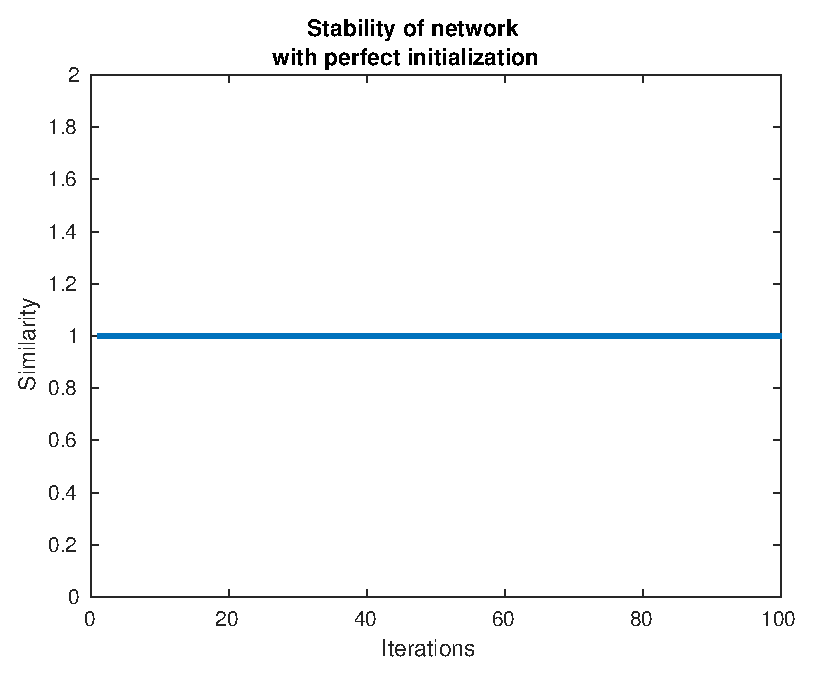
\includegraphics[width=\textwidth]{figs/stable}
        \caption{By initializing the network to the stored pattern, the network will remain in an equilibrium. The network will never deviate from this state without external interference. If the network is initialized to a noisy state, the network will converge towards the stored pattern.}
    \end{subfigure}
    \begin{subfigure}{0.49\textwidth}
        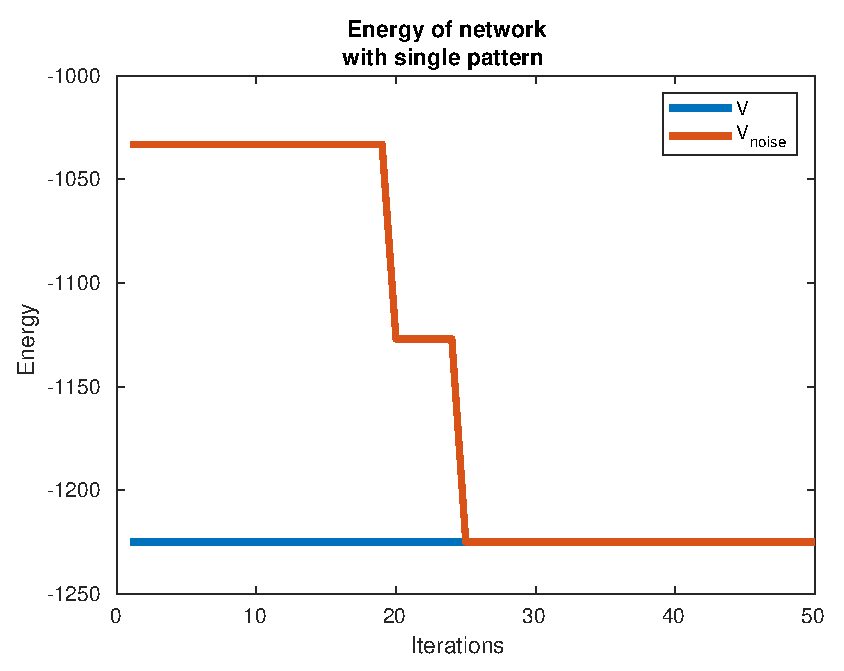
\includegraphics[width=\textwidth]{figs/stable-energy}
        \caption{With a single stored pattern, the energy will converge towards the lower limit according to \cref{eq:energy-limits}. In this case with 50 neurons, the lower limit is $-\frac{50*\times 49}{2} = -1225$}.
    \end{subfigure}
    \caption{Initializing a Hopfield network with a single stored pattern ($N = 50$) will cause the network to converge towards the stored pattern.}
    \label{fig:stable}
\end{figure}
To test whether the Hopfield network is stable after reaching an equilibrium we simulated the Hopfield network storing a random pattern using $N=50$ neurons. We initialized the network to the stored pattern, once with and once without added noise, as shown in \cref{fig:stable}. The network remained stable at the equilibrium point, and converged towards the equilibrium if not perfectly intialized. With a single pattern stored, the energy converged toward the lower limit expressed in \cref{eq:energy-limits}.

\subsection{Storing multiple patterns}
\begin{figure}[H]
    \centering
    \captionsetup[subfigure]{width=0.9\textwidth, justification=raggedright}
    \begin{subfigure}{0.49\textwidth}
        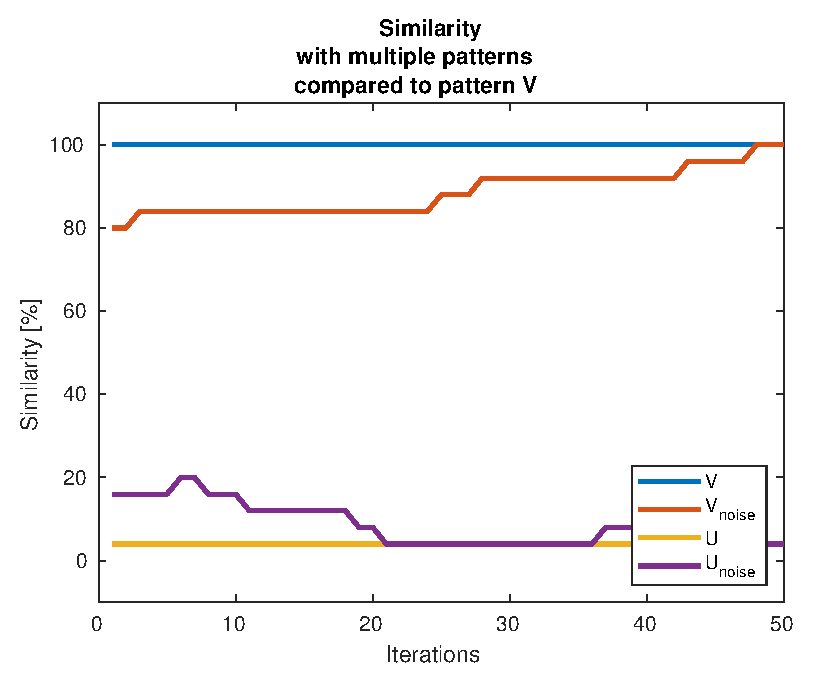
\includegraphics[width=\textwidth]{figs/multiple-patterns.eps}
        \caption{By initializing the weight matrix $\bf W$ with multiple patterns, the network is able to restore multiple different patterns. The amount of memories and noise the network is able to handle depends on the size and similarity of the stored patterns. If two stored patterns only differ by a few bits, the network may recall the wrong memory if noise is involved. }
        \label{fig:multiple-similarity}
    \end{subfigure}
    \begin{subfigure}{0.49\textwidth}
        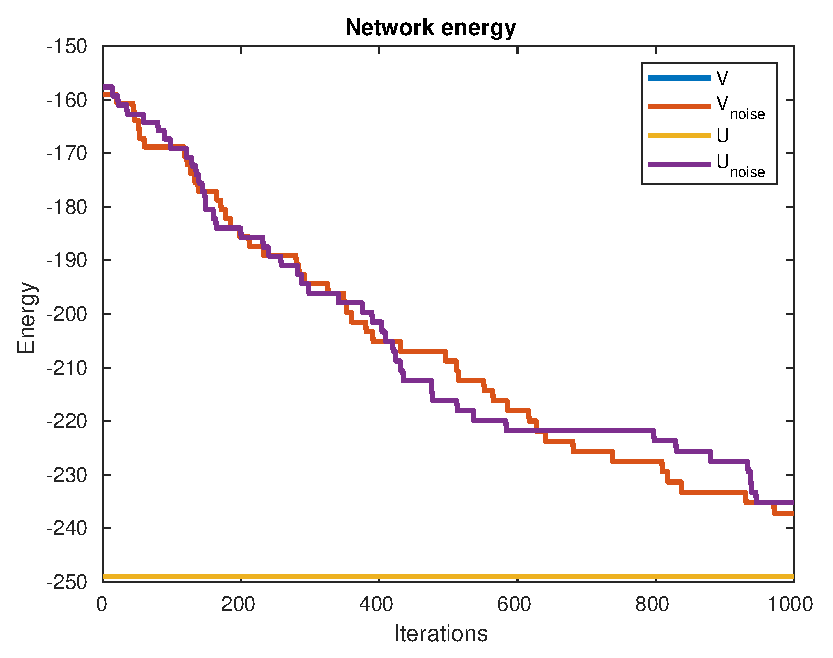
\includegraphics[width=\textwidth]{figs/multiple-patterns-energy.eps}
        \caption{The network will always move in the direction of least resistance such that the overall energy decreases, similar to how a ball will always roll downwards into a valley unless there are external forces interfering. Each stored memory corresponds to a local minimum which can be thought of as a valley. As long as the network is initialized to the correct valley, it is able to reconstruct the stored pattern from memory.}
        \label{fig:multiple-energy}
    \end{subfigure}
    \begin{subfigure}{0.49\textwidth}
        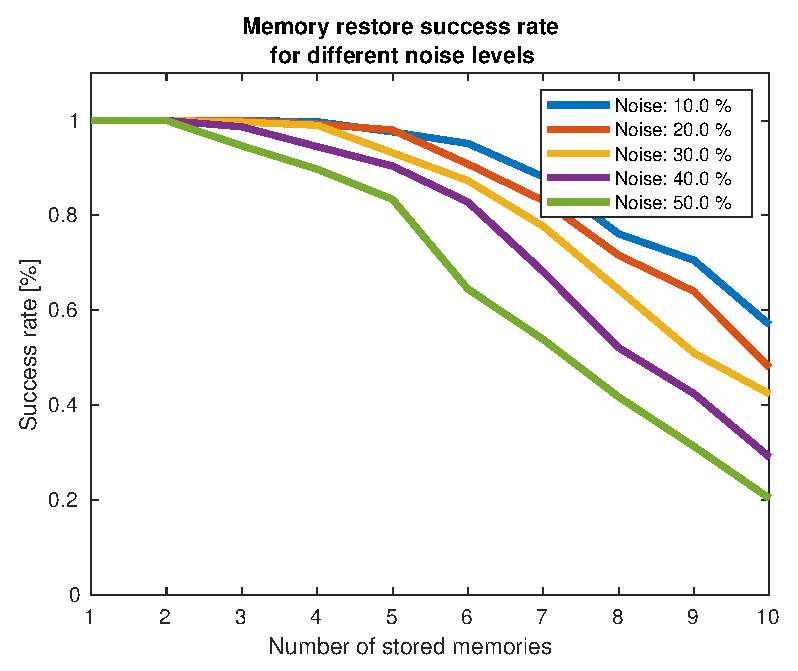
\includegraphics[width=\textwidth]{figs/capacity.eps}
        \caption{When storing a large amount of random patterns in the network, the robustness decreases and the network will not be able to reliably restore the correct memories. The figure shows the proportion of correct memories, recalled for different number of stored memories and different noise levels.}
        \label{fig:multiple-capacity}
    \end{subfigure}
    \caption{Simulating the Hopfield network with multiple stored patterns.}
    \label{fig:multiple}
\end{figure}
To test whether the network remains stable even with multiple patterns stored in the weights, we simulated a new network storing two uncorrelated random patterns ($N=50$). We simulated using both patterns as initial conditions as well as simulating with and without noise. In total we ran 4 simulations and the results are shown in \cref{fig:multiple}. The states converged towards the correct pattern in all cases, and remains stable at the equilibrium. The energy in the equilibrium, as shown in \cref{fig:multiple-energy}, was half the lower limit in \cref{eq:energy}.

To test how many pattern we can reliably store, we simulated the Hopfield with different number of memories and noise levels. In \cref{fig:multiple-capacity} we see how the networks ability to recall the correct memory decreaes as both the number of memories and noise level increases. With low noise levels we found that we can store $6$ memories reliably using $N=50$ neurons. For higher noise levels the robustness quickly decreases.
 

\subsection{Reconstructing partial QR codes from memory} \label{sec:qr-codes}
To better visualize the Hopfield networks ability to store and restore patterns, we constructed a Hopfield network for storing QR-codes. We stored two QR-codes in the network and initialized the network with only partial information. Fig. \ref{fig:qr-codes} shows how the network was able to restore the correct QR code from memory, while \cref{fig:qr-codes-stability} shows how the network remained stable after reaching the equilibrium. 
\begin{figure}[H]
    \centering
    \captionsetup[subfigure]{width=0.9\textwidth, justification=raggedright}
    \begin{subfigure}{0.49\textwidth}
        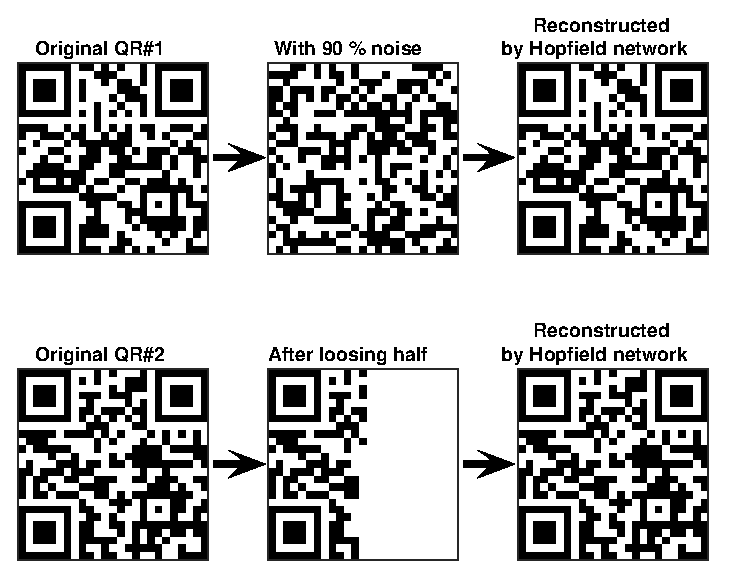
\includegraphics[width=\textwidth]{figs/qr-code}
        \caption{The QR-code contains information encoded within the patterns. A QR decoding app, either online or on a smartphone, can be used to decode the "hidden" message. Using the Hopfield network we are able to reconstruct a destroyed QR-code from memory.}
        \label{fig:qr-codes}
    \end{subfigure}
    \begin{subfigure}{0.49\textwidth}
        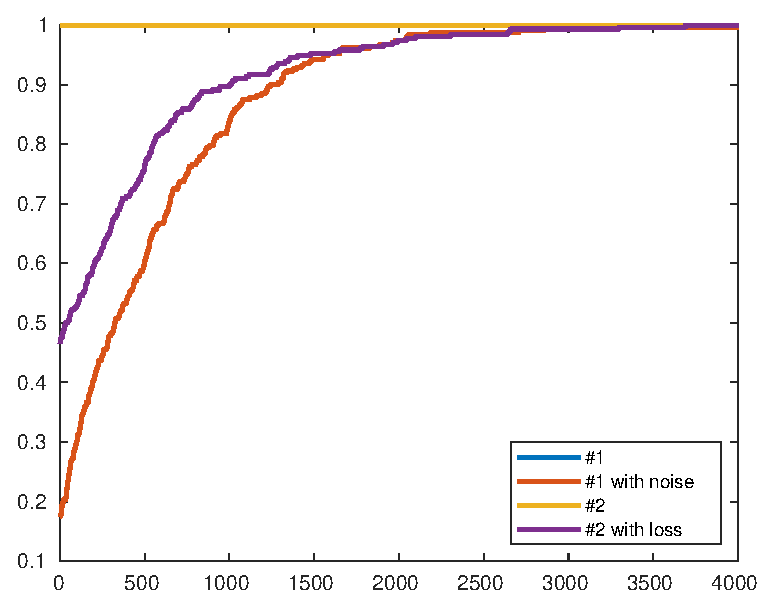
\includegraphics[width=\textwidth]{figs/qr-code-sim}
        \caption{The similarity between the current state of the network and the original QR-code we want it to reconstruct.}
        \label{fig:qr-codes-stability}
    \end{subfigure}
    \caption{By applying the Hopfield network to a very noisy QR-code we are able to reconstruct the original. By using any QR-code reader we are able to decode the original and reconstructed QR-codes, while the middle ones contain too much noise. The same Hopfield network was used to reconstruct both patterns.}
\end{figure}

\subsection{Inverting patterns}
According to the weights, \cref{eq:weights}, the Hopfield network only stores patterns and not the actual values in the memories. A pattern $\bf V$ and its inverse $\mathbf{\bar{V}} = -1 \times \bf V$ would yield the exact same weight matrix. For each stored memory there should be two equilibrium states, one for $\bf V$ and one for $\bf \bar{V}$. To test whether this truly is the case, we used the same Hopfield network as in \cref{sec:qr-codes} and initialized the states to the second QR code, but inverting all bits. We ran another simulation using the QR-code with two-thirds of its bits inverted. As can be seen from the results in \cref{fig:inverted-qr} both cases caused the Hopfield network to reconstruct the inverted pattern, and not the ones we originally created. This shows how for each stored pattern there exists two equilibrium points.
\begin{figure}[H]
    \centering
        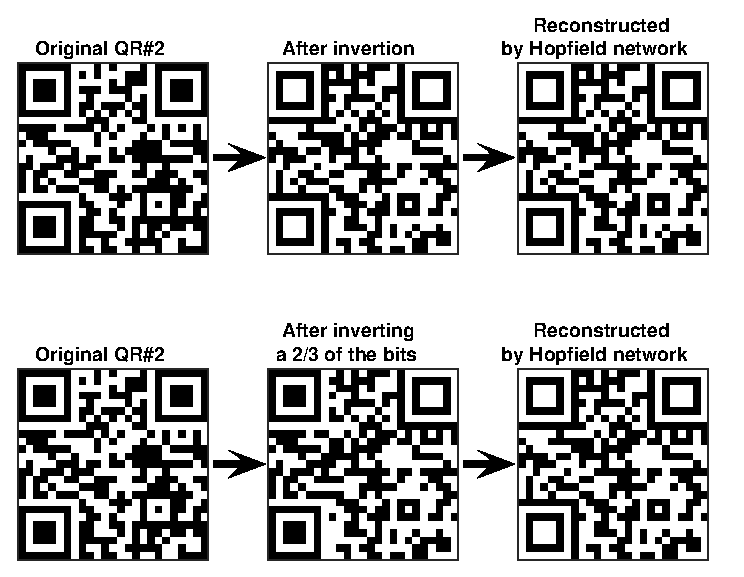
\includegraphics[width=0.5\textwidth]{figs/qr-inverted}
        \caption{The Hopfield network learns the patterns and the network is not able to distinguish between positive and negative values. The network is not only stable at the initial memories, but also when using the inverted patterns.}
        \label{fig:inverted-qr}
\end{figure}